Sprinkler-pumpe systemet består af en Hunter PS Pop-up sprinkler og en Alpha 2 pumpe fra Grundfoss, disse forbindes med passende slanger og fittings. For at styre sprinkleren, skal Alpha 2 pumpen kunne tændes og afbrydes. Dette gøres via et 230V/5V relæ. Dette relæ styres via én pin Enheden. 

\subsection{Driver}

Driveren der skal håndtere Sprinkler-pumpe systemet, skal kunne aktivere/deaktivere det forudbestemte sprinklerrelæ. Metoden modtager en adresse parameter samt en on/off parameter. Herefter sætter metoden en af den forudbestemte pin på Enheden høj/lav (3.3V/0V). Herefter søger relæstyringen og 230V/5V relæet for hhv. tænde/slukke for sprinkleren. 


\subsubsection*{Pseudokode}

\begin{lstlisting}[language=C]
void controlSprinkler(int address, bool on_off){
Manage Sprinkler address
Activate/deactivate corresponding Sprinkler
}
\end{lstlisting}



\subsection{230V/5V relæ}

For at 230V/5V relæet kan blive en realitet, er det pålagt, at dette bygges i en lukket kasse og godkendes af en elektronikværksteds-ansvarlig. Kassen som bygges har et 230Vac apparatstik ind og et 230Vac stikkontakt ud. For at skabe forbindelse/afbrydelse af denne 230Vac strøm benyttes et relæ, dette relæ styrers af 5V. Når 5V  tilføjes relæets spole, klikker relæet og der skabes gennemgang fra apparatstik til stikkontakt. Dette lukkede kredsløb bygges som sagt ind i en lukke kasse med gennemsigtigt låg. Relæet der benyttes er et Finder 40.52s Figuren \ref{lab:RELAY} viser kredsløbet for dette lukkede kredsløb.

\begin{figure}[H] \centering
{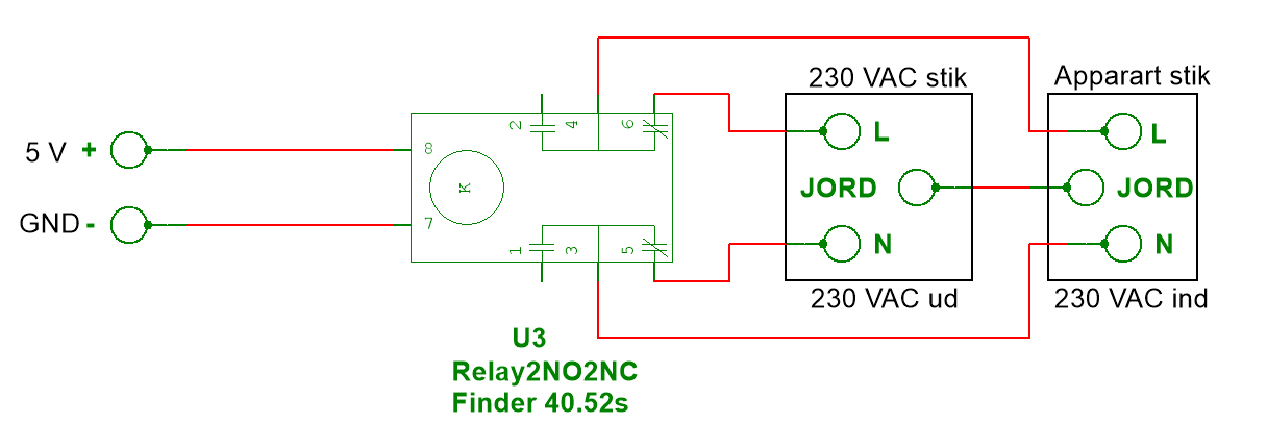
\includegraphics[width=\textwidth]{filer/design/Billeder/230VAC_KREDS}}
\caption{230V/5V relæ}
\label{lab:RELAY}
\raggedright
\end{figure}

\subsection{Alpha 2 pumpen}

Alpha 2 pumpen skal blot tilsluttes 230Vac + jord. Der medfølger et special stik til selve pumpen, dette forbindes til en 230V stikprop, med 3-ledet kabel (Leder, Nul og Jord) . Stikproppen kan nu sættes i 230V/5V relæets 230V stikkontakt.

\begin{figure}[H] \centering
{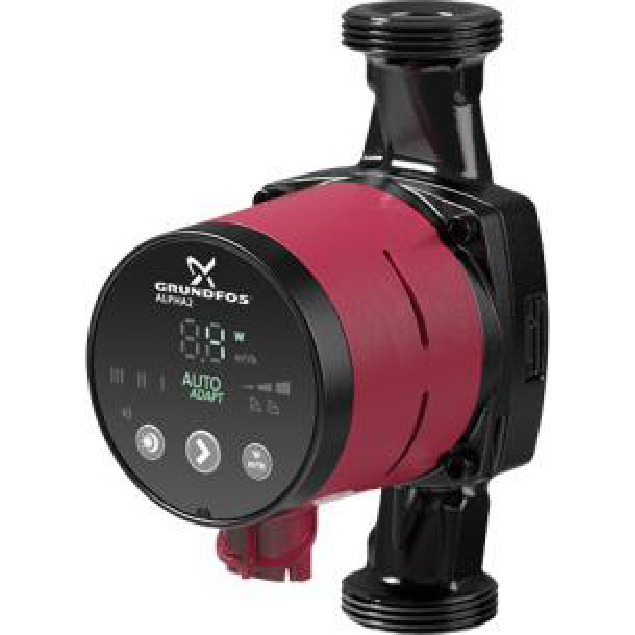
\includegraphics[width=0.4\textwidth]{filer/design/Billeder/Alpha2}}
\caption{Alpha2 Cirkulationspumpe fra Grundfoss}
\label{lab:Alpha2}
\raggedright
\end{figure} 

\subsection{Relæ styring}

I følge databladet for Finder 40.52s (figur \ref{lab:finder4052s}), kræver relæet 100mA ved 5V forsyning, som databladet

\begin{figure}[H] \centering
{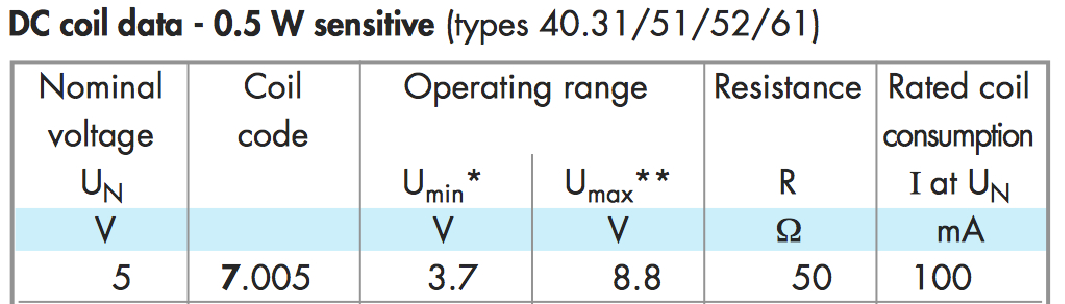
\includegraphics[width=0.7\textwidth]{filer/design/Billeder/finder4052s}}
\caption{Datablad for Finder 40.52s - 100mA}
\label{lab:finder4052s}
\raggedright
\end{figure} 

PSoC'ens udgang giver hverken størm eller spænding nok til at trække relæet. PSoC'en afgiver 3,3V og relæet kræver 5V. For at opnå dette benyttes en transistor til styringen af relæet. Relæet kræver 5V og 100mA, Derfor skal transistoren opfylde dette krav. Det gør BC547 

\begin{figure}[H] \centering
{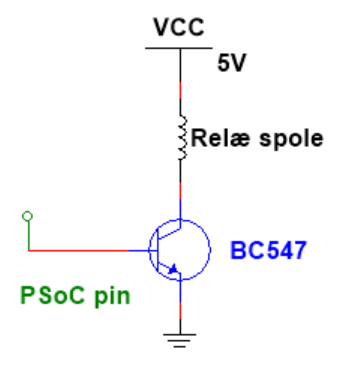
\includegraphics[width=0.3\textwidth]{filer/design/Billeder/BC547}}
\caption{BC547 opsætning}
\label{lab:BC547}
\raggedright
\end{figure} 

Når PSoC'ens pin til BC547 transistoren går høj (3,3V), så skabes der forbindelse mellem collector og emittier på transistoren, herved er der 5V over relæets spole og relæets kontaktsæt klikker herved. 





 